\chapter{Math Gallery Collection 2}

\section{Overview}

\begin{figure}[H]
    \centering
    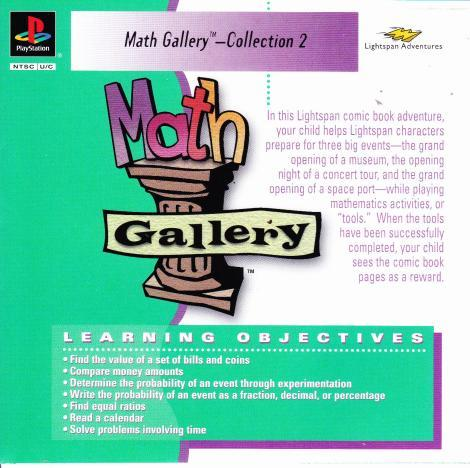
\includegraphics[width=0.5\textwidth]{Games/MathGalleryCollection/Images/MathGalleryCollection2Cover.jpg}
    \caption{Official Math Gallery: Collection 2 CD Cover}
\end{figure}

Math Gallery: Collection 2 features four different types of math for the player to choose from:

\begin{itemize}
    \item Ratio
    \item Money
    \item Time
    \item Probability
\end{itemize}

\section{Transcripts}

\subsection{Series 10}

\subsubsection{Introduction}

Ginger: Leaping lollipops, guys! The museum grand opening celebration is tonight and there's still so much to do!

Mars the Moose: Don't worry, Ginger, we'll help!

Pink Animal: Yeah, Mars and I'll search the island for more objects to display in the museum while you take care of things here.

Ginger: Alright, I have the master plan.

\subsubsection{Clip 1}

Pink Animal: Hey Ginger, now we're off the hook! Look what I found!

Ginger: Jumping jelly beans! I have just the place for them!

\subsubsection{Clip 2}

Mars the Moose: Check out this apple! It's the one Snow White ate.

Ginger: Wow, Mars, it'll be the core of our foodstuffs exhibit.

\subsubsection{Clip 3}

Mars the Moose: Ginger, look what Peter Pan donated to the museum!

Ginger: That is beyond the shadow of a doubt the best exhibit item yet!

\subsubsection{Clip 4}

Ginger: Tumbling taffy, we're ready for the grand opening celebration just in time!

Mars the Moose: Yeah, and check out all the famous Fairy Tale Island characters.

Rapunzel: Well, yes, I do go through a lot of shampoo.

Princess 1: These hors d'oeuvres are too hot.

Princess 2: Well, I just couldn't sleep. There was this horrid lump in my mattress.

Man 1: Yes, I have changed my diet quite a bit. I used to eat like such a beast.

Ginger: Attention everyone! Thanks for joining us this evening. It is now time to unveil the masterpiece of our new museum collection: The Emperor's New Clothes.

\subsection{Series 20}

\subsubsection{Introduction}

Small Grey Dog (Gershwin): Well this is it - opening night of our Calculating Canines tour.

Female Dog (Ella): I can't wait to see our set designs come to life!

Daphne: Yep, and Yorkshires, I'm so glad I found you guys! One of the trucks has been delayed - the one with all of your props.

Large Brown Dog: Whoa!

Daphne: And there is still so much to do to get ready!

Large Grey Dog: Hey, we can get paints and brushes! Yeah, lots of brushes, and we'll make new props ourselves!

Female Dog (Maxine): Stand back, the artiste is here!

Daphne: I have the master plan. Let's do it!

\subsubsection{Clip 1}

Large Brown Dog: Whoa Max, you're a regular Pug-casso!

Female Dog (Maxine): Ha ha!

\subsubsection{Clip 2}

Large Grey Dog: Whoa, I guess I need to brush up on my painting skills. Ha ha! Woah.!

\subsubsection{Clip 3}

Female Dog (Ella): Hey guys, it's ready! The perfect prop for our song "Barking in the USA".

Small Grey Dog (Gershwin): Bwow, great! It's Mount Rushmore!

\subsubsection{Clip 4}

Female Dog (Ella): I'ma rockin' and rollin' bow wow wow!

Max: Hey Ella, you're really on a roll!

Ella: Oh!

\subsubsection{Clip 5}

Announcer: Ladies and gentlemen, K95!

Male Dogs (singing): Searching for answers.

Female Dogs (singing): Putting on a chase.

Male Dogs (singing): Looking everywhere.

All Dogs (singing): All over the place! Left, right, up, down, everywhere across the town! North, west, all around, [figure till we find the town!] Dig it up, drop it down. Dig it up, yeah! Dig it up, track it down, yeah!

\subsection{Series 30}

\subsubsection{Introduction}

Space Port Operator: The Spaceport grand opening celebration is tonight! Splendiferous space travelers will be anxiously arriving soon.

Gracie: Terrific! I'm ready! Start the party!

Space Port Operator: But we're not finished stocking the station.

Ryan: Gracie and I will help.

Space Port Operator: That's great news! I have a meticulous master plan right here.

\subsubsection{Clip 1}

Gracie: How many robots does it take to screw in all these light bulbs? Just one.

\subsubsection{Clip 2}

Gracie: Oh, we got a load of marshmallows!

Ryan: Hehe, good thing it wasn't a crate of watermelons!

\subsubsection{Clip 3}

Gracie: Gee, what's in here? Boy, looks like we're really in a pickle now.

\subsubsection{Clip 4}

Ryan: The grand opening is a success. We finished just in time.

Space Port Operator: Yes, copious crowds continue to arrive every minute.

Ryan: Who will be providing the entertainment?

Space Port Operator: You'll see. Welcome everyone. Tonight we have a special musical guest. Please give a hand for Groovy Gracie and her Galactic Guitars!

\section{Credits}

Concept by: Margy Hillman, Liz Herrick;
Story written by: Liz Herrick;
Vice President, Development Operations: David Adams;
Vice President, Curriculum and Product Design: Liz Herrick;
Program Managers: Heidi Janzen, Alma Torres, Darlene Tschudy;
Lead Content Designers: Janet Clark, Kelly Robinson;
Content Designers: Linda Bussell, Amy Nicholson, Ann Rybowiak, Kimberley Tatman;
Senior Program Manager of Curriculum: Sherri Furqueron;
Lead Curriculum Specialist: Jacqueline Gianola-Quinn;
Curriculum Writers: Paz A. Lacsamana-Jensen, Janice Morton, Tim Scheidt;
Editor: Helen Hansen;
Curriculum Consultants: Nicholas Branca Ph.D., Judith Jacobs Ph.D., Teri Perl Ph.D.;
Interactive Game Coordinator: Kristin Rix, Janene Wittmayer;
Director, Curriculum Support and Assessment: Judy Carr, Linda Paulson;
Curriculum Support: Candace Hodges;
Writer: John Dorsey;
Lead Desktop Publisher: Leslie Braznell;
Vice President, Studio Production: Joanne Odenthal, Ph.D.;
Executive Producer: David Hamby;
Animation Director: Al Lowenheim;
Interactive Producer: David Adams;
Associate Producers: Jennifer Mah Hindman, Jo Anne Palasi;
Production Manager: Janet Dahle;
Director, Media Production Technologies: Scott Murdoch;
Assistant Art Director: Ken Anderson;
Unit Manager, Preproduction and 2-D: Jan Hastings;
Assistant Directors: Burt Vincent Julio, Rosemary Horvath, Luther McLaurin, Jeff Merghart, Steve Merghart, Virgil Sanico;
Unit Manager, Interactive: Eydie Gilley;
Background Artist: Edgardo Magsino;
Lead Game Artists: Byron Rodarmel, Callie Mack;
Graphic Artists: Sean Jackson, Dan Jones;
3-D Manager/Senior Compositor: Eric Fuss;
Unit Manager, Post Production and 3-D: Colleen McPhillips;
Audio Producer: Rick Bowman;
Audio Engineers: Brad Aldredge, Chris Jahnkow;
Video Assistant: Keith Marcussen;
Voice Talent: Eileen Bowman, Deem Bristow, Deanna Driscoll, Deanna Hurst, Ron Jones, Paul James Kruse, Royal Lihzis, Mike Lowe, Lani Minella, Deborah Washington;
Asset Management Supervisor: Monica Chernus;
Production Control Technician: David Martin;
Technical Editors: Sandy Mazur, Lori Silfen;
Data Management Assistant: Sjoukie Cooper-Holt;
Asset Management Archivist: Katharine Laxa;
Executive Administrator: Rae Farley;
Vice President, Software Development: Sergio Garcia;
Director, Product Development: Bob Warren;
Lead Software Engineer: Janet Academia;
Programmers: Scott Quiggle, Bae Yu;
Production Assistant: Tonette Salter;
Quality Assurance Manager: Mark Myers;
Quality Assurance Supervisors: Jenna Payne, Fred Pecoroni;
Quality Assurance Analysts: James Cajala, Darren Craun, Parish Goynes, David Hickson, Rives Jones, Janet Row, Geno Vici;
Quality Assurance Testers: Johnny Carter, Mark Champlin, Kevin Garcia, John Gruber, Barbara King, Ines Panchenko, Kathy Taylor, Marlan Wilson, Cyrille Zarate, John Zimmerman;

\clearpage
\newpage

\section{Screenshots}

\begin{figure}[H]
    \centering
    \begin{subfigure}{0.45\textwidth}
        \centering
        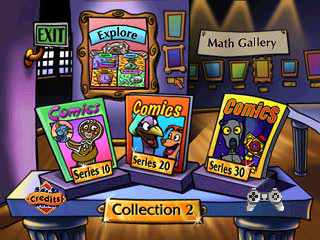
\includegraphics[width=\linewidth]{Games/MathGalleryCollection/Images/MathGalleryCollection2Image1.png}
        \caption{Math Gallery: Collection 2 - Screenshot 1}
    \end{subfigure}
    \begin{subfigure}{0.45\textwidth}
        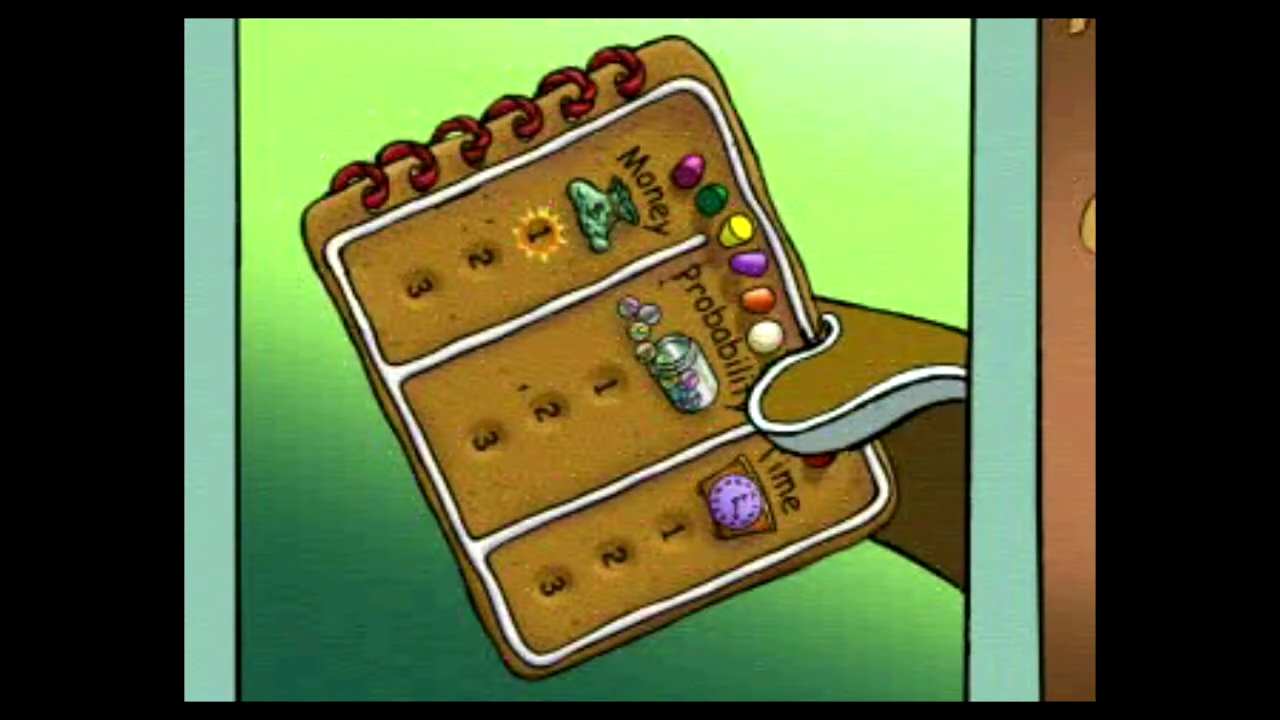
\includegraphics[width=\linewidth]{Games/MathGalleryCollection/Images/MathGalleryCollection2Image2.png}
        \caption{Math Gallery: Collection 2 - Screenshot 2}
    \end{subfigure}

    \begin{subfigure}{0.45\textwidth}
        \centering
        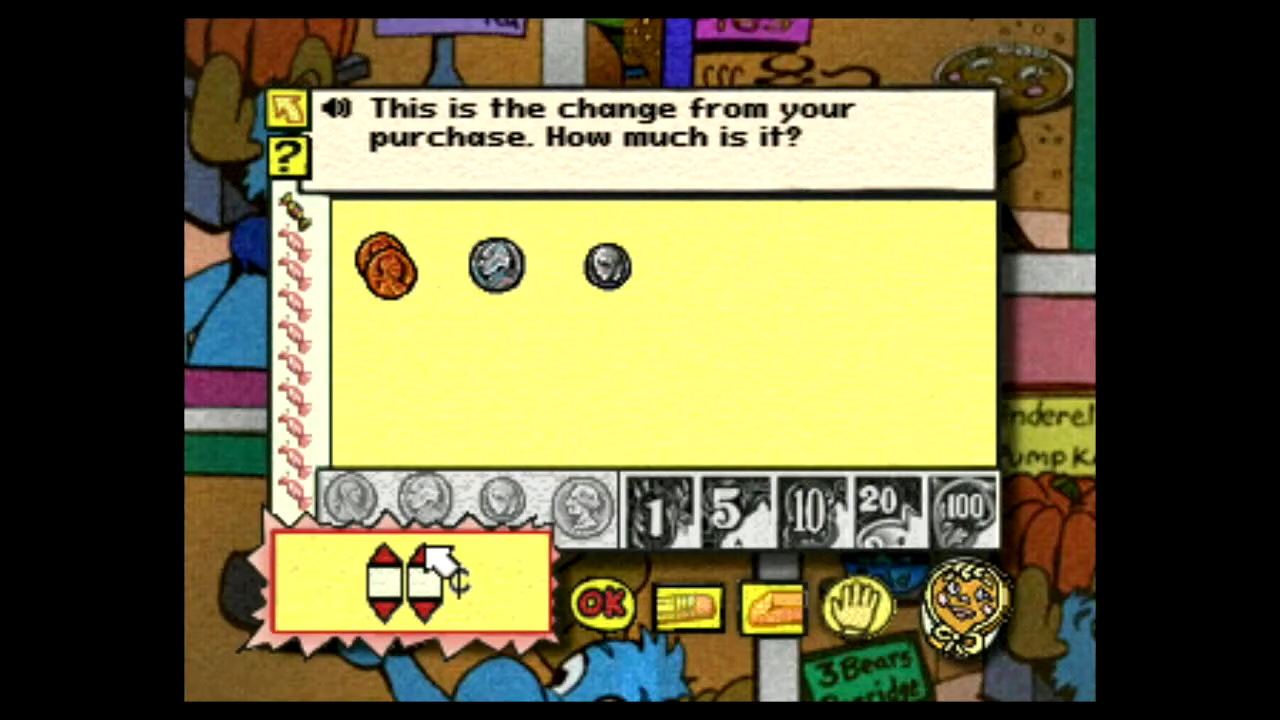
\includegraphics[width=\linewidth]{Games/MathGalleryCollection/Images/MathGalleryCollection2Image3.png}
        \caption{Math Gallery: Collection 2 - Screenshot 3}
    \end{subfigure}
    \begin{subfigure}{0.45\textwidth}
        \centering
        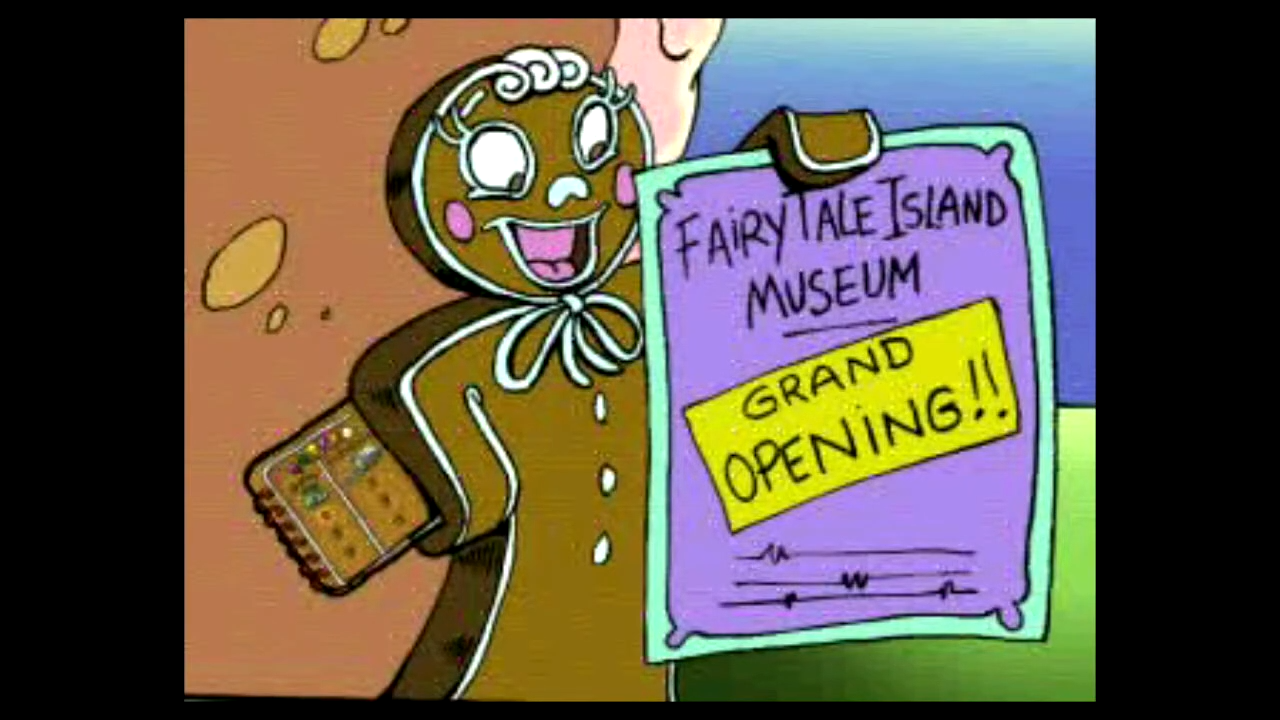
\includegraphics[width=\linewidth]{Games/MathGalleryCollection/Images/MathGalleryCollection2Image4.png}
        \caption{Math Gallery: Collection 2 - Screenshot 4}
    \end{subfigure}
    \caption{Screenshots from Math Gallery: Collection 2}
\end{figure}